% id: 16-13
% book: 베이직쎈 확률과 통계 · 01 여러 가지 순열
% section: 유형 009 최단 거리로 가는 경우의 수
% figure: tikz:fig-16-13
% answer: 
% answer_source: 
% variant_level: 0 (원본 전사)
% 이 파일은 build.mjs 가 items.json 에서 만든다. 고칠 때는 items.json 을 고친다.
\smash{\raisebox{1.5mm}{\dmkichul{베이직쎈 확률과 통계 16쪽 13번}}}
\noindent\begin{minipage}[t]{0.58\linewidth}\vspace{0pt}\raggedright 오른쪽 그림과 같은 도로망이 있다. $\pt{A}$에서 $\pt{P}$를 거쳐 $\pt{B}$까지 최단 거리로 가는 경우의 수는?\end{minipage}\hfill\begin{minipage}[t]{0.4\linewidth}\vspace{0pt}\centering \resizebox{\ifdim\width>\linewidth\linewidth\else\width\fi}{!}{% 16-13(본책 16쪽) — 가로 5칸·세로 4칸 도로망(A 왼쪽 아래 · B 오른쪽 위 · P 는 오른쪽 2칸·위 1칸 지점). 스캔 그림을 TikZ 로 다시 그림(스캔 화질).
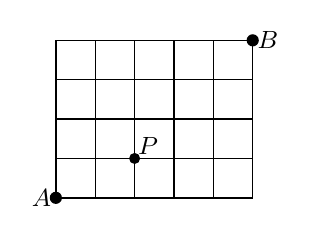
\begin{tikzpicture}[line width=0.5pt]
  \foreach \x in {0, 0.5, 1, 1.5, 2, 2.5} { \draw (\x,0) -- (\x,2); }
  \foreach \y in {0, 0.5, 1, 1.5, 2} { \draw (0,\y) -- (2.5,\y); }
  \fill (0,0) circle (2.2pt);
  \node[left, font=\small, inner sep=1.5pt] at (0,0) {$\pt{A}$};
  \fill (2.5,2) circle (2.2pt);
  \node[right, font=\small, inner sep=1.5pt] at (2.5,2) {$\pt{B}$};
  \fill (1,0.5) circle (2pt);
  \node[above right, font=\small, inner sep=1pt] at (1,0.5) {$\pt{P}$};
\end{tikzpicture}
}\end{minipage}\par
\dmchoicesauto{}{$48$}{$51$}{$54$}{$57$}{$60$}
